
\section{Introduction}
\label{sec:intro}

Knowledge Base Question Answering (KBQA) leverages the rich semantic information in Knowledge Bases (KB) to deeply understand natural language questions and provide precise answers. Since KBQA holds significant value in applications such as search engines, intelligent healthcare, and financial risk control~\citep{jang2017kbqa, wu2024medical, chen2025ifqa}, it has garnered extensive attention in recent years. Although KBQA performs well on simple questions, it still struggles with complex questions in real-world scenarios. This difficulty primarily arises from generalizing to a wide range of unseen complex questions and adapting to the heterogeneous structures of KBs.

\begin{figure*}
    \centering
    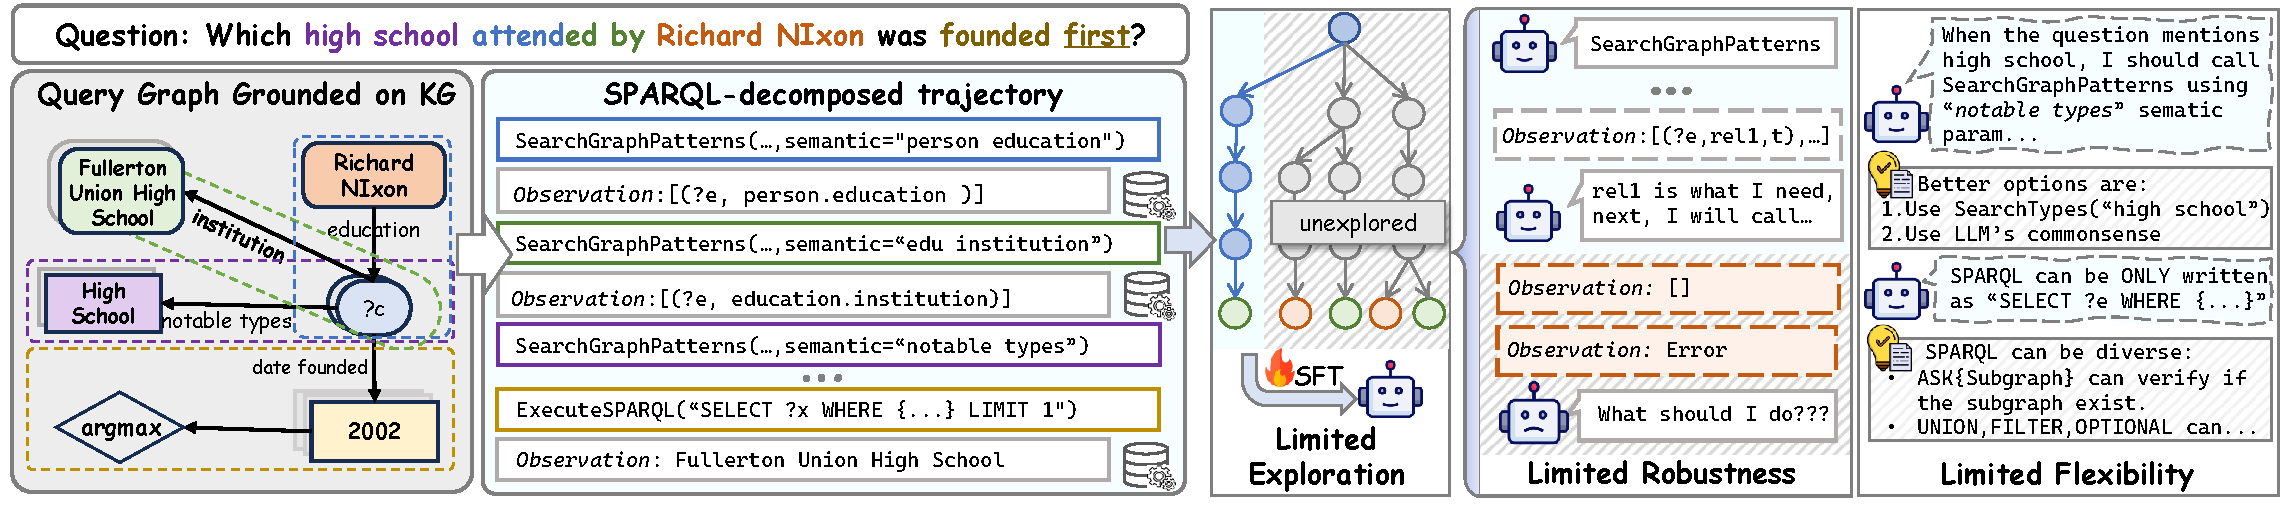
\includegraphics[width=1\textwidth]{figures/intro.pdf}
    \caption{The key limitations of existing agentic approaches that rely on process supervision. }
    \label{fig:intro}
\end{figure*}

Existing semantic-parsing-based~\citep{shu2022tiara, jiangunikgqa} and information-retrieval-based KBQA approaches~\citep{liu2022graftnet, sun2019pullnet} rely on predefined workflows (e.g., generate-then-retrieve or retrieve-then-rank pipelines), resulting in error propagation and adaptability limitations. Recently, a series of approaches has adopted an agentic reasoning paradigm. As illustrated in the middle of Fig.~\ref{fig:intro}, under this paradigm, LLMs autonomously perform task planning, tool calling, and ultimately derive precise answers through multi-turn interactions with KBs. Specifically, existing agentic approaches fall into two categories, i.e., prompting-based~\citep{xiong2024interactive, sunthink} and finetuning-based approaches~\citep{jiang2024kgagent, fang2024dara, zhu2025knowagent}. The former uses hand-crafted few-shot prompts to guide reasoning, relying on the intrinsic reasoning ability of LLMs. However, few examples are inadequate for the model to understand complex questions, perceiving the KB structure, resulting in low performance. In response, finetuning-based approaches adapt open-source LLMs by constructing agentic reasoning trajectories and fine-tuning the model to follow them. However, most of them rely on process supervision. Since manually creating high-quality trajectories is labor-intensive, they typically synthesize reasoning trajectories by decomposing gold logical forms (e.g., SPARQL). Besides, they learn from trajectories via Supervised Fine-Tuning (SFT) to employ the model with agentic reasoning ability. 
%Some recent work~  \citep{luokbqao1, xiong2025mcts} further augments trajectories using Monte Carlo Tree Search (MCTS). However, they still rely heavily on process supervision. 

Despite the progress, existing finetuning-based approaches rely heavily on process supervision both in data generation and model training. They encourage LLMs to exploit idea trajectories rather than autonomously exploring alternative ones. Consequently, they have two critical limitations: 
\begin{itemize}[leftmargin=*]
\item  \textbf{Limited Robustness.} Under process supervision, as shown in the left part of Fig. \ref{fig:intro}, training trajectories are typically decomposed from gold logical forms, with each step being idealized and error-free. However, such trajectories omit the noise and uncertainty inherent in real-world interactions. As a result, models always struggle when exposed to the noisy, such as tool-call failures and empty results, as they are trained on ideal trajectories. 
\item \textbf{Limited Flexibility.} For many questions, there exists more than one correct trajectory, and in some cases, certain trajectories may even outperform the gold logical forms. Training on trajectories only derived from gold logical forms constrains the model to low-diversity behavioral patterns. As shown in Fig.~\ref{fig:intro}, when the model is presented with an example problem containing a``high school'' type constraint, it insists on finding a predicate with the meaning ``notable type'' and applies the type constraint. However, more efficient solutions exist, such as leveraging common sense to identify entities of a specific type from the candidate set, or using ``SearchTypes'' to more directly constrain the entity types.
\end{itemize}

% In this paper, we propose \ours, an LLM that can autonomously perform agentic reasoning on KBs to obtain answers. To incentivize autonomous exploration, \ours\space trains the LLM under outcome-only supervision via a multi-stage curriculum reinforcement learning with an easy-to-hard curriculum. To establish foundational agentic capabilities, \ours\space first fine-tunes the LLM on a small set of high-quality trajectories obtained through outcome-based rejection sampling. Then, to alleviate the reward sparsity inherent in outcome-only supervision, it applies multi-stage curriculum RL with reward schedules that progress from easy to hard.

Motivated by this, in this paper, we propose \ours, an LLM capable of autonomously performing task decomposition, invoking tools, refining formal queries, and executing them to obtain answers. To incentivize autonomous exploration, \ours\space adopts a multi-stage curriculum reinforcement learning approach that relies mainly on outcome supervision. First, to break free from the dependency on process annotation, it employs an outcome-based rejection sampling strategy to curate high-quality trajectories and perform to endow the model with a foundational exploration capability. To mitigate the reward sparsity induced by outcome-only signals, \ours\space employs multi-stage curriculum RL on reward schedules that progress from easy to hard, steadily strengthening autonomous exploration and complex reasoning. Trained with only around 6700 outcome-supervised samples, \ours\space consistently outperforms previous agentic KBQA approaches across three mainstream datasets, i.e., WebQSP, CWQ, and GrailQA. Using \textbf{12×} less training data, it achieves an F1 score of 80.5\% on GrailQA, achieving a \textbf{3.3\%} relative improvement over KBQA-o1, the previous SOTA agentic-based approach. Notably, on the zero-shot subset of GrailQA, \ours\space achieves a relative improvement of up to \textbf{11.1\%} compared to KBQA-o1, demonstrating the strong generalization ability of the proposed approach.


In summary, our contributions are as follows:
\begin{itemize}
    % \item We propose \ours, a novel multi-stage reinforcement learning paradigm that successfully incentivizes agentic reasoning capabilities using only outcome supervision.
    \item  We propose \ours, our first agentic reasoning model for KBQA. Relying mainly on outcome supervision, it learns to act as a robust and flexible agent, capable of recovering from errors and strategically exploring diverse reasoning trajectories.

    % \item \ours \space first establishes a foundational agentic capability via a cold-start finetuning phase, then strengthens autonomous exploration with a curriculum RL in reward criteria from easy to hard while discouraging reward hacking.
    \item To address the reward sparsity inherent in outcome-only supervision, we propose a multi-stage curriculum reinforcement learning with an easy-to-hard curriculum, progressing from easy to hard reward criteria while discouraging reward hacking.
    
    % \item Experiments on three mainstream datasets demonstrate that under a low-resource setting, using only question-answer pairs, especially in more challenging scenarios, such as zero-shot settings.
    \item Extensive experiments on three mainstream datasets demonstrate that \ours\space consistently outperforms previous agentic KBQA approaches, particularly in challenging zero-shot scenarios.
\end{itemize}